\chapter{Background Information}

Gait velocity estimation using pHRI depends two main components - modeling human walking and then using those models in an estimator. The models used in the estimator may be physics based or data-driven. Gait may be modeled using passive physics-based models such as the Bipedal Spring-Loaded Pendulum (B-SLIP) \cite{geyer2006compliant,liu2015dynamic} model. A passive model does not have any active control inputs to modify gaits and as steady-state human walking is periodic, optimization methods need to be used to find periodic model gaits. Periodicity is ensured in the resulting gaits by using Poincar\'e maps in the gait optimization \cite{strogatz2018nonlinear,garcia1998simplest}.

\section{Poincar\'e maps}

A Poincar\'e section for a dynamical is a subspace that has fewer dimensions that the model's state space. For the B-SLIP model, it may be placed at a gait event such as midstance (MS), touchdown (TD), or lift-off (LO) when the value of one of the states may be fixed e.g., when the vertical velocity of the \COM is zero. Let the Poincar\'e section be placed at MS, and let $ \mathcal{P} $ of the state $ \x_k $ be a function that returns the state after one cycle, or a step in the case of the B-SLIP, such that $ \x_{k+1} = \mathcal{P}(\x_k) $. The function $ \mathcal{P}(\x_k) $ is the Poincar\'e map and there exists an initial state representing a periodic orbit where the initial state maps back to itself after one period such that

\begin{equation}
	\x_k = \mathcal{P}(\x_k)
\end{equation}

\begin{figure}
	\centering
	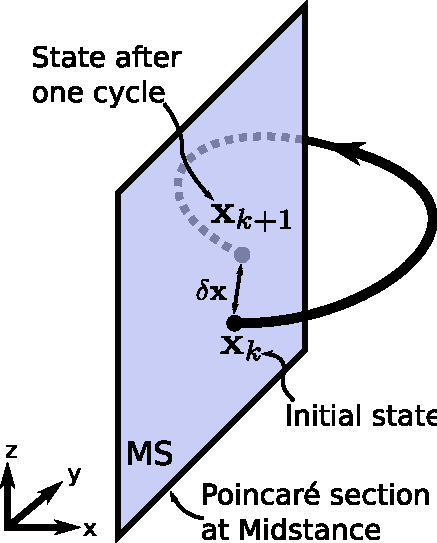
\includegraphics[width=.3\linewidth]{poincare.pdf}
	\caption{A Poincar\'e map used to find periodic gaits}\label{fig:poincare}
\end{figure}

A Poincar\'e section placed at MS is shown in blue in Fig.~\ref{fig:poincare}. The dynamics of the model are integrated for one step using $ \x_k $ as the initial condition. Optimization methods are used to find initial conditions that yield periodic gait by minimizing $ \delta \x $, the error between $ \x_k $ and $ \x_{k+1} $. The nonlinear return map may be linearized about these periodic gaits for further refining the gait search as described in Chapter \ref{chapter:IMM}. Model gaits for various velocities may be used as references while estimating an exoskeleton user's desired gait. Measurements of quantities such as CoM height and velocity, may be compared to simulated model gaits using state estimation tools such as the Kalman filter.

\section{Kalman filters for state estimation}

Kalman filtering is a feedback-based sequential optimal state estimation technique \cite{kalman1960new}. The filter is initialized at a certain initial state estimate $ \hat{\x}_0 $ that may have associated uncertainty due to measurement errors. The evolution of this state is described using dynamical system presented in the following equations
%
\begin{eqnarray}
	\dot{\x}(t) &=& \mathbf{f}(\x(t),\u(t),\mathbf{w}(t),t),\quad \mathbf{w}(t) \sim \mathcal{N}(0, \Q(t))  \label{eq:sys}  \\
	\tilde{\y}_k &=& \mathbf{h}(\x_k) + \mathbf{v}_k,\quad \mathbf{v}_k \sim \mathcal{N}(0,\R_k) \nonumber
\end{eqnarray}
%
\noindent where $ \x(t) $ and $ \u(t) $ are the continuous-time states and inputs, $ \y_k $ are the discrete-time measurements, and $ \mathbf{f}(\x(t),\u(t),t) $ and $ \mathbf{h}(\x_k) $ are the system and measurement function respectively. The system has zero-mean Gaussian process and measurement noises $ \mathbf{w}(t) $ and $ \mathbf{v}_k $ respectively with covariances $ \Q(t) $ and $ \R_k $ respectively. The measurement noise $ \mathbf{w}(t) $ is combined with the measurement equation $ \mathbf{h}(\x_k) $ to form the noisy measurement $ \tilde{\y}_k $. 

\begin{figure}
	\centering
	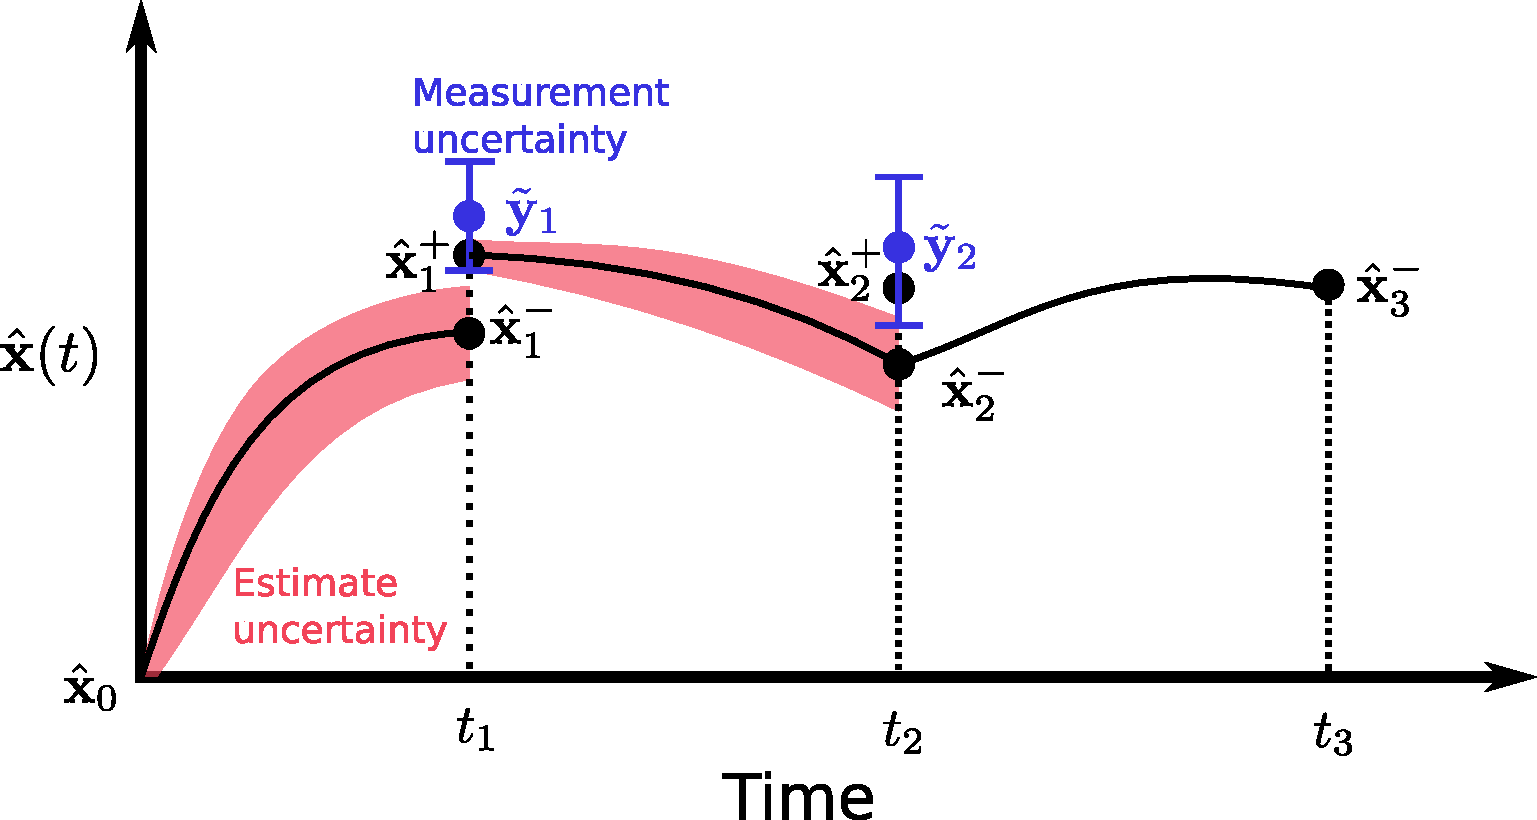
\includegraphics[width=0.7\linewidth]{kalman.pdf}
	\caption{Illustration of the Kalman Filtering process}\label{fig:kalman}
\end{figure}

The uncertainty of the estimates $ \hat{\x} $ increases as the state is propagated forward through time using the system dynamics. Regular measurements of state variables are used to reduce the uncertainty and increase the accuracy of the estimates as illustrated in Fig.~\ref{fig:kalman} where the $ + $ and $ - $ in the superscript denote pre- and post-update states. Kalman filters account for both, the uncertainty in the state estimates and in the measurements. Further details of this process are as follow.

The state estimates and estimate covariance $ \P $ are propagated in continuous time such that
\begin{eqnarray}
	\dot{\hat{\x}} &=& \mathbf{f}(\hat{\x},\u,t) \\
	\dot{\P}(t) &=& \F(t)\P(t) + \P(t)\F^T(t) + \mathbf{G}(t)\Q(t)\mathbf{G}(t)^T \\ 
	\F(t) &\equiv& \frac{\partial \mathbf{f}}{\partial \x} \Bigr |_{\hat{\x}(t),\u(t)} \nonumber
\end{eqnarray}


\noindent The states are sequentially updated such that
\begin{eqnarray}
	\K_k &=& \P_k^- \H^T_k(\hat{\x}_k^-) \left[\H_k(\hat{\x}_k^-)\P_k^- \H^T_k(\hat{\x}_k^-) + \R_k\right]^{-1} \\
	\hat{\x}_k^+ &=& \hat{\x}_k^- + \K_k[\tilde{\y}_k-\mathbf{h}(\x_k)] \\
	\P_k^+ &=& [\mathbf{I} - \K_k \H_k(\hat{\x}_k^-)]\P_k^-,\quad \H_k(\hat{\x}_k^-) \equiv \frac{\partial \mathbf{h}}{\partial \x} \Bigr |_{\hat{\x}_k^-}
\end{eqnarray}

\noindent where $ \K_k $ is the Kalman gain, $ \F(t) $, and $ \H_k(\hat{\mathbf{x}}_k^-) $ are the linearized dynamics and measurement model respectively. The updated estimates and their covariance are $ \mathbf{x}_k^+ $ and $ \mathbf{P}_k^+ $ respectively. The above equations describe a Continous-Discrete Kalman filter setup. System dynamics are propagated in continuous time but states are updated in discrete time since measurements are discrete.
